\section{Os Axiomas da Substituição}
Nesta seção, veremos que toda boa ordem é isomorfa a um único número ordinal.
Para isso, precisamos introduzir um novo axioma, o \emph{axioma da substituição}.

Pelo Exercício \ref{ex:uniao-boas-ordens}, o conjunto $\{0\}\times \omega\cup\{1\}\times \omega$ é, com a ordem lexicográfica, uma boa ordem.


% no preâmbulo:
% \usepackage{tikz}
\begin{figure}[h]
    \centering
    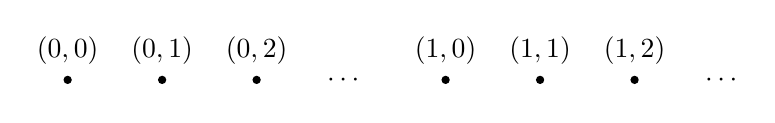
\begin{tikzpicture}[baseline=(current bounding box.center)]
        % sequência {(0,n) : n \in \omega}
        \foreach \x/\lab in {
            0/{$(0,0)$},
            1.2/{$(0,1)$},
            2.4/{$(0,2)$}
        }{
            \fill (\x,0) circle (1.5pt);
            \node[above=2pt] at (\x,0) {\lab};
        }
        \node at (3.5,0) {$\cdots$};

        % sequência {(1,n) : n \in \omega}
        \foreach \x/\lab in {
            4.8/{$(1,0)$},
            6.0/{$(1,1)$},
            7.2/{$(1,2)$}
        }{
            \fill (\x,0) circle (1.5pt);
            \node[above=2pt] at (\x,0) {\lab};
        }
        \node at (8.3,0) {$\cdots$};
    \end{tikzpicture}
    \caption{A boa ordem $\{0\}\times \omega\cup\{1\}\times \omega$ com a ordem lexicográfica.}
\end{figure}

Como representaríamos tal boa ordem através de um ordinal?

Ora, $\omega$ é isomorfo à boa ordem $\{0\}\times \omega$.
$S(\omega)=\omega+1$ é isomorfo à boa ordem $\{0\}\times \omega\cup\{1\}\times \{0\}$.
$S(S(\omega))=\omega+2$ é isomorfo à boa ordem $\{0\}\times \omega\cup\{1\}\times \{0, 1\}$ e
``\emph{assim por diante}''.

Podemos formalizar isso formalmente, com os axiomas que temos.
Para tanto, gostaríamos de introduzir, por definição, um símbolo de função $S(n, x)=S^n(x)$ tal que:
\begin{itemize}
    \item $S^0(x)=x$;
    \item $S^{n+1}(x)=S(S^n(x))$
\end{itemize}

Para tanto, podemos utilizar a seguinte definição:

\begin{definition}
    Seja $G$ um símbolo de função binário introduzido por definição tal através da seguinte expressão:

    \[
    G(t, x)=\begin{cases}
    x & \text{se } t \text{ é função e } \dom t=0,\\
    S(t(n)) & \text{se } t \text{ é função e } \dom t=n+1 \text{ para algum } n\in \omega,\\
    \emptyset & \text{caso contrário.}
    \end{cases}
    \]

    Define-se $S^n(x)=y$ se, e somente se, $n\notin \omega$ e $y=\emptyset$, ou $n \in \omega$ e existe uma função $t$ tal que $n+1\subseteq \dom t$ e, para todo $m\in n+1$, $t(m)=G(t|m, x)$, e $t(n)=y$.
\end{definition}

Como na demonstração do Teorema da Recursão para $\omega$, prova-se que para todo $n\in \omega$ e $x \in \omega$, existe $t$ tal que $n+1\subseteq \dom t$ e, para todo $m\in n+1$, $t(m)=G(t|m, x)$, e que se $t, t'$ são duas tais funções, então $t=t'$.
Não escreveremos estes detalhes, pois, em breve, descreveremos um resultado mais geral.

Assim, $S^n(x)$ é bem definido para todo $n\in \omega$ e $x\in \omega$.
Podemos, ainda, definir $\omega+n=S^n(\omega)$ para todo $n\in \omega$.

A ideia, agora, é que $\omega+\omega=\bigcup\{\omega+n : n\in \omega\}$ é um ordinal isomorfo à boa ordem $\{0\}\times \omega\cup\{1\}\times \omega$.
Porém, há um problema fundamental: não é possível, com os axiomas que temos, provar que $\{S^n(\omega) : n\in \omega\}$ é um conjunto.

Também não é possível afirmar que existe uma função $F$ de domínio $\omega$ tal que $F(n)=S^n(\omega)$ para todo $n\in \omega$.
A operação $\omega\rightarrow \omega+n$ consiste na introdução, por um processo de definição, de uma \emph{símbolo de função} $F$ tal que $F(n)=S^n(\omega)$ para todo $n\in \omega$, da mesma forma que $S$ é um símbolo de função introduzido por definição tal que $S(x)=x\cup\{x\}$ para todo conjunto $x$.
Tais símbolos fazem parte da linguagem, mas não denotam conjuntos.

O \emph{esquema de  axiomas da substituição} é um axioma introduzido por Fraenkel que garante que, sob condições análogas às de $F$ (cujo domínio ``seria um conjunto''), mas não às de $S$ (cujo domínio ``não seria comportado por um conjunto''), tais funções existem.

\begin{axiom}[Esquema de axiomas da substituição]
    Para cada fórmula $\phi(x, y, A, t_1, \dots, t_n)$, a seguinte fórmula é um axioma.
    \[
        \forall t_1, \dots, t_n \forall A \left( \forall x\in A \exists! y \phi(x, y, A, t_1, \dots, t_n) \rightarrow \exists B \forall y (\exists x\in A \phi(x, y, A, t_1, \dots, t_n)\rightarrow y \in B)\right).
    \]
\end{axiom}
Com esse axioma, é possível garantir que para todo $t$, $\{S^n(t) : n\in \omega\}$ é um conjunto. Para tanto,
considere a fórmula $\phi(x, y, A, t)$ dada por $y=S^n(t)$.
Então 
\[
    \forall t \forall A \left( \forall n\in A \exists! y \phi(n, y, A, t_1, \dots, t_n) \rightarrow \exists B \forall y (\exists n\in A \phi(n, y, A, t_1, \dots, t_n)\rightarrow y \in B)\right).
\]
Fixado $t$ e posto $A=\omega$, temos que $\forall n\in \omega \exists! y S^n(t)=y$, e, assim, existe um conjunto $B$ tal que $\forall y (\exists n\in \omega S^n(t)=y\rightarrow y \in B)$.

Agora, pelo axioma da compreensão, podemos tomar o conjunto $\{y\in B : \exists n\in \omega S^n(t)=y\}$, cujos elementos são exatamente os $S^n(t)$ para $n\in \omega$.

Esta etapa da compreensão pode ser sistematizada como se segue:

\begin{proposition}[Esquema da substituição compreendida]
    Para cada fórmula $\phi(x, y, A, t_1, \dots, t_n)$, a seguinte fórmula é um teorema
    \[
        \forall t_1, \dots, t_n \forall A \left( \forall x\in A \exists! y \phi(x, y, A, t_1, \dots, t_n) \rightarrow \exists B \forall y (\exists x\in A \phi(x, y, A, t_1, \dots, t_n)\leftrightarrow y \in B)\right).
    \]
\end{proposition}
\begin{proof}
    Sejam dados $t_1, \dots, t_n$ e $A$ tais que $\forall x\in A \exists! y \phi(x, y, A, t_1, \dots, t_n)$.
    Pelo axioma da substituição, existe um conjunto $B'$ tal que $\forall y (\exists x\in A \phi(x, y, A, t_1, \dots, t_n)\rightarrow y \in B')$.

    Seja $B=\{y\in B' : \exists x\in A \phi(x, y, A, t_1, \dots, t_n)\}$.
    Então,
    \[
    \forall y (\exists x\in A \phi(x, y, A, t_1, \dots, t_n)\leftrightarrow y \in B).
    \]
\end{proof}

Vamos ainda aprimorar a nossa notação um pouco mais a partir de símbolos de função.
\begin{definition}
    Seja $F(x, t_1, \dots, t_n)$ um símbolo de função introduzido por definição,de modo que para alguma fórmula $\phi(x, t_1, \dots, t_n, y)$, temos
    \[
        \forall t_1 \dots \forall t_n \forall A \forall x \exists! t \phi(x, t_1, \dots, t_n, y)
    \]
    e
    \[
       \forall t_1 \dots \forall t_n \forall A \forall x \Bigl( F(x, t_1, \dots, t_n)=y \leftrightarrow \phi(x, t_1, \dots, t_n, y)\Bigr).
    \]

    Então, dados $t_1, \dots, t_n, A$,
    o único conjunto $B$ tal que $\forall y (\exists x\in A \phi(x, t_1, \dots, t_n, y)\leftrightarrow y \in B)$ é denotado como se segue:
    
    \[
        F_{t_1, \dots, t_n}[A]=\{F(x, t_1, \dots, t_n) : x\in A\}.
    \]

    Além disso, $f: A\to B$ tal que $\forall x\in A (f(x)=F(x, t_1, \dots, t_n))$ é denotada por $F_{t_1, \dots, t_n}|A$.
\end{definition}
Observação: na definição acima, a fórmula $\phi$ não é obrigada a ter parâmetros $t_1, \dots, t_n$.
Neste caso, simplesmente utilizamos as notações $F[A]$ e $F|A$.

De posse do esquema dos axiomas da substituição, podemos provar que toda boa ordem é isomorfa a um único número ordinal.

\begin{theorem}
    Para toda boa ordem $A$, existe um único número ordinal $\alpha$ tal que $A$ é isomorfo a $\alpha$.
\end{theorem}
\begin{proof}
    A unicidade vem da Proposição \ref{prop:ordinais-nao-isomorfos}.
    
    Para a existência, seja $F(P, a)$ um símbolo de função introduzido por definição como se segue:
    \[
        F(P, a)=\begin{cases}
        \alpha & \text{se } \exists A, <\,\Big(P=(A, <) \text{ é uma boa ordem e } a\in A \text{ e } \alpha \text{ é um ordinal isomorfo à } A[a]\Big),\\
        \emptyset & \text{caso contrário.}
        \end{cases}
    \]

    Dada uma boa ordem $P=(A, <)$, seja $X=\{a \in A : \exists \alpha \text{ ordinal isomorfo à } A[a]\}$.
    Seja $\alpha=F_p[X]$ e $f=F_p|X$.

    $f$ é uma função crescente e $X$ é um segmento inicial:
    com efeito, dado $b \in X$ e $a<b$ em $A$, seja $\beta$ um ordinal isomorfo à $A[b]$.
    Seja $g: A[b]\to \beta$ um isomorfismo.
    Então $g|A[a]: A[a]\to \beta[f(a)]$ é um isomorfismo.
    Note que $f(a)=\beta[f(a)]=\{\xi \in \beta: \xi<f(a)\}=f(a)$.
    Assim, $a\in X$ e $f(a)<f(b)$.

    Além disso, $\alpha$ é um ordinal.
    Como $\alpha$ é um conjunto de ordinais, basta ver que $\alpha$ é transitivo.
    Para tanto, tome $\beta\in \alpha$ e $\xi\in \beta$.
    Seja $b\in X$ tal que $F_p(b)=\beta$.
    Seja $g: A[b]\to \beta$ um isomorfismo, e seja $a\in A$ tal que $g(a)=\xi$.
    Então $g|A[a]: A[a]\to \xi$ é um isomorfismo, de modo que $a\in X$ e $F_p(a)=\xi$.
    Assim, $\xi\in \alpha$.

    Como $f: X\to \alpha$ é estritamente crescente e sobrejetora, $f: X\to \alpha$ é um isomorfismo.
    Se $X$ for um segmento inicial próprio de $A$, escreva $X=A[a]$ para algum $a\in A$.
    Temos que $a \notin X$.
    Porém, $f:A[a]\to \alpha$ é um isomorfismo, de modo que $a \in X$, um absurdo.

    Assim, $X=A$ e $f: A\to \alpha$ é um isomorfismo.
\end{proof}